\documentclass[10pt,a4paper]{article}
\usepackage[utf8]{inputenc} % para poder usar tildes en archivos UTF-8
\usepackage[spanish]{babel} % para que comandos como \today den el resultado en castellano
\usepackage{a4wide} % márgenes un poco más anchos que lo usual
\usepackage[conEntregas]{caratula}
\usepackage{ulem}
\usepackage{amsmath} 
\usepackage{amssymb}
\usepackage{fancybox}
\usepackage[usenames,dvipsnames]{color}
\usepackage{hyperref}
\usepackage{listings}
\usepackage{clrscode3e}
\usepackage{xcolor}
\usepackage{amsmath}
\usepackage{arydshln}
\usepackage{listings}

\hypersetup{
    colorlinks,
    citecolor=black,
    filecolor=black,
    linkcolor=black,
    urlcolor=black
}

\lstdefinestyle{customc}{
  belowcaptionskip=1\baselineskip,
  breaklines=true,
  frame=L,
  xleftmargin=\parindent,
  language=C,
  showstringspaces=false,
  basicstyle=\footnotesize\ttfamily,
  keywordstyle=\bfseries\color{green!40!black},
  commentstyle=\itshape\color{purple!40!black},
  identifierstyle=\color{blue},
  stringstyle=\color{orange},
}

\lstset{escapechar=@,style=customc}

\begin{document}

\titulo{Trabajo Práctico 2}
\subtitulo{[Primera entrega]}

\fecha{\today}

\materia{Bases de Datos}
\integrante{Fernandez, Esteban}{691/12}{esteban.pmf@gmail.com}
\integrante{Marta, Cristian G.}{079/12}{cristiangmarta@gmail.com}
\integrante{Wright, Carolina Rocío}{876/12}{wright.carolina@gmail.com}

\maketitle

\tableofcontents
\newpage

\section{Introducción}
Continuaremos el desarrollo del Sistema de seguimiento de casos policiales. Agregaremos una base de datos NoSQL basada en documentos (MongoDB) para guardar el historial de los casos. De esta forma podremos hacer consultas de manera más eficiente.

\section{Diseño NoSql}
Basándonos en el diseño entregado en el Trabajo Práctico 1, hemos creado el siguiente diagrama que refleja el contenido de los documentos que utilizaremos para realizar las consultas.

\begin{figure}[h]
	\centering
	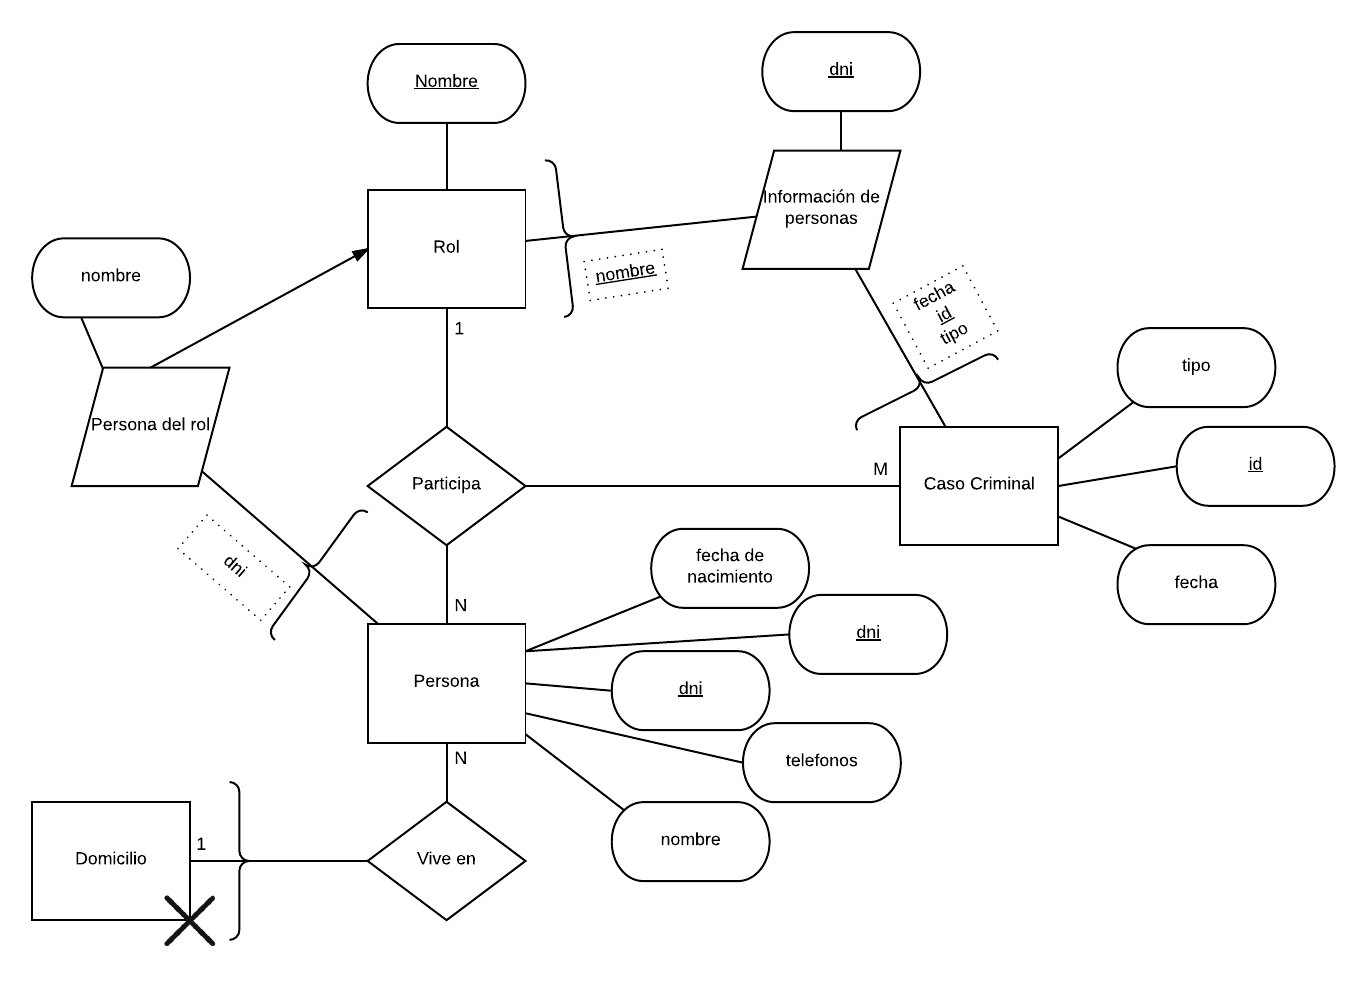
\includegraphics[width=\linewidth]{imagenes/DID.png}
\end{figure}

\subsection{JSON schemas}

\subsubsection{Persona}
\begin{lstlisting}
{
	dni: 36949514,
	fecha_nacimiento: 10/11/1992,
	nombre: "Carolina",
	apellido: "Wright", 
	domicilio: {
		id: 1,
		numero: 5950,
		calle: "20 de febrero"
	}
}
\end{lstlisting}

\subsubsection{Persona de rol}
\begin{lstlisting}
{ 
  [
    {
      nombre_rol: "Testigo"
      personas: [
              {
            		dni_persona: 36949514,
            	},
              {
              	dni_persona: 36949515,
            	}
          ]
  },
  {
    nombre_rol: "Culpable"
    personas: [
              {
              	dni_persona: 36949516,
            	},
              {
              	dni_persona: 36949517,
            	}
          ]
  }
  ]
  
}
\end{lstlisting}

\subsubsection{Información de personas}
\begin{lstlisting}
{
  [
    {
  		dni_persona: 36949514,
  		
  		caso_y_rol: [
        {
         id: 2,
          fecha_ingreso: 31/10/2016,
    		  fecha: 29/10/2016,
    		  lugar: "Palermo",
    		  descripcion: "Robo de billetera",
    		  nombre_categoria: "Robo",
    		  estado: "Pendiente"
        },
        {
          id: 3,
      	  fecha_ingreso: 31/09/2016,
    		  fecha: 29/11/2016,
    		  lugar: "Belgrano",
    		  descripcion: "Robo de auto",
    		  nombre_categoria: "Robo",
    		  estado: "Pendiente"
        }
        ]
  	},
    {
    	dni_persona: 36949632,
  		
  		caso_y_rol: [
        {
          id: 3,
          fecha_ingreso: 31/10/2016,
    		  fecha: 21/03/2016,
    		  lugar: "Retiro",
    		  descripcion: "Robo de banco",
    		  nombre_categoria: "Robo",
    		  estado: "Resuelto"
        },
        {
          id: 5,
      	  fecha_ingreso: 31/09/2016,
    		  fecha: 22/11/2016,
    		  lugar: "Barracas",
    		  descripcion: "Secuestro",
    		  nombre_categoria: "Robo",
    		  estado: "Resuelto"
        }
        ]
  	}
  
  ]
	
}

\end{lstlisting}

\subsubsection{Rol}
\begin{lstlisting}
{
	nombre: "Testigo"
}
\end{lstlisting}


\subsubsection{Caso criminal}
\begin{lstlisting}
{
	  id: 1,
	  fecha_ingreso: 31/10/2016,
	  fecha: 29/10/2016,
	  lugar: "Palermo",
	  descripcion: "Robo de billetera",
	  nombre_categoria: "Robo",
	  estado: "Pendiente"
}
\end{lstlisting}

\section{Parte 2 - Map Reduce}

\end{document}